\begin{figure}[htp]
    \centering
    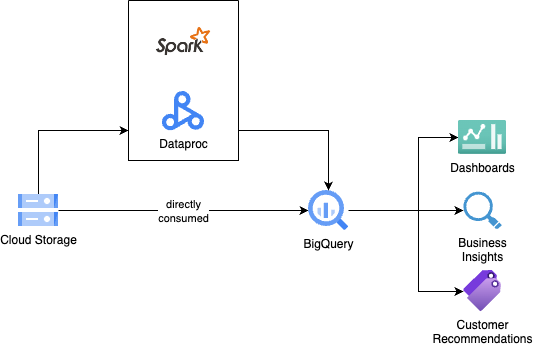
\includegraphics[width=0.5\linewidth]{images/solution_architecture.png}
    \caption{Overview of Solution Architecture}
\end{figure}

Our team's primary objective focused on developing a sophisticated data pipeline architecture
designed to efficiently process and analyze retail data at scale. The core workflow encompasses the
transformation of raw retailer-provided data into actionable insights within Google BigQuery, our
selected data warehouse solution. This implementation supports two critical business functions:
first, the generation of \textbf{Personal Product Ranking} (PPR) - a comprehensive recommendation
tagging system that leverages historical transaction data to provide personalized product
suggestions; and second, the creation of detailed temporal analysis visualizations that track sales
performance across multiple time dimensions. The architecture was specifically designed to handle
large-scale retail data processing while maintaining data integrity and ensuring optimal query
performance for downstream analytical applications.

The technical implementation begins with the assumption that retailers upload their raw data files
to Google Cloud Storage, chosen for its robust object storage capabilities and seamless integration
with other Google Cloud Platform services. Our architectural approach incorporates a comparative
analysis of two distinct data ingestion methodologies: the traditional Apache Spark ETL pipeline,
widely recognized for its distributed processing capabilities, versus native BigQuery data loading
commands, which leverage BigQuery's serverless architecture. This dual-implementation strategy
allows for a comprehensive evaluation of performance metrics, cost efficiency, and architectural
complexity between these approaches. The ingestion processes are meticulously designed to handle
various data formats and volumes, with both pathways ultimately populating BigQuery tables that
serve as the foundation for our customer recommendation engine. These recommendations are
systematically computed and stored in dedicated BigQuery tables, optimized for quick retrieval and
regular updates to maintain recommendation relevancy.

Product Personalized Recommendation (PPR) involves suggesting products to customers based on their
historical purchasing data from various channels like POS machines and digital platforms. By
analyzing comprehensive purchase histories, retailers can develop sophisticated algorithms that
predict consumer interests, enabling more intelligent stocking strategies and maximizing profit
potential. The rise of e-commerce has made such data-driven approaches crucial, allowing businesses
to create personalized digital engagement platforms that recommend products during key customer
journey moments like product searches and checkout.

These customer recommendation systems leverage advanced machine learning techniques to transform raw
purchasing data into valuable insights, helping retailers optimize inventory, reduce waste, and
create more targeted marketing approaches. By implementing intelligent product tagging and
personalization strategies, businesses can enhance customer experiences, improve conversion rates,
and gain deeper understanding of consumer behavior across both online and offline shopping
environments.

For visualization requirements, our team adopted a streamlined approach by leveraging BigQuery Data
Canvas, a built-in visualization tool within the BigQuery ecosystem. This strategic decision was
driven by considerations of system integration, operational efficiency, and ecosystem cohesion. By
utilizing native BigQuery capabilities, we eliminated common challenges associated with third-party
visualization solutions, such as authentication complexity, data synchronization issues, and
potential security vulnerabilities. The seamless integration with BigQuery's existing infrastructure
ensures consistent performance and reliability while maintaining robust data governance standards.

The implementation of BigQuery Data Canvas significantly enhanced our data exploration and
visualization workflow. Data scientists and analysts can directly interact with warehouse data,
creating visualizations and conducting exploratory analysis without the overhead of managing
additional software licenses or external tool dependencies. This native integration provides
substantial benefits for resource optimization by eliminating the need for data export processes or
intermediate storage solutions typically required for external visualization tools. Furthermore, the
tool's capability for real-time data visualization directly from BigQuery tables enables immediate
insight generation and validation, particularly valuable for iterative analysis processes where
rapid feedback loops between data exploration and visualization are essential.